\chapter{Firewall}

The goals of this assignment include the following.

\begin{itemize}
\item Familiarizing ourselves with firewalls.
\item Correctly configuring the different options.
\item Configuring a local area network, establishing different security polices using filtering and traffic monitoring.
\item Solve a case study about connecting an SME network to the Internet using a firewall.
\end{itemize}

\section{Home preparation}

Read from the following document:
\url{www.jaumebarcelo.info/teaching/lxs/ipsec/ASA_Getting_Started.pdf}
all the assignments, and prepare a solution for the \emph{case study}.

\section{Configuring the working place}
Each group needs 3 PCs and a Cisco ASA 5505 firewall.

One of the PCs will be connected to the patch panel.
Before disconnecting this PC from the Internet, download an FTP server (e.g. Filezilla)
The other two, are connected to the two internal ports of the firewall.

The firewall and the external PC will be connected to the patch panel and switch B.
The external IP of the firewall will be configured according to the figure (where X is the group number).
Configure the default gateway of the PCs with the corresponding firewall interface (internal for the internal PCs and external for the external PCs).

\begin{figure}
\centering
\ifpdf
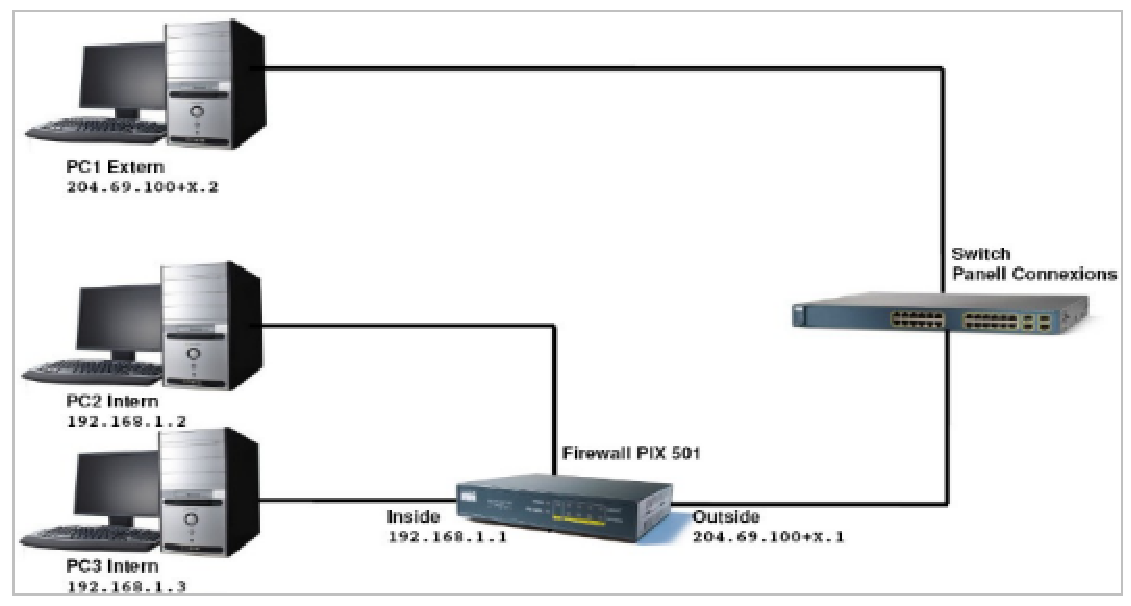
\includegraphics[width=0.9\linewidth]{Figures/firewall_topology.pdf}
\else
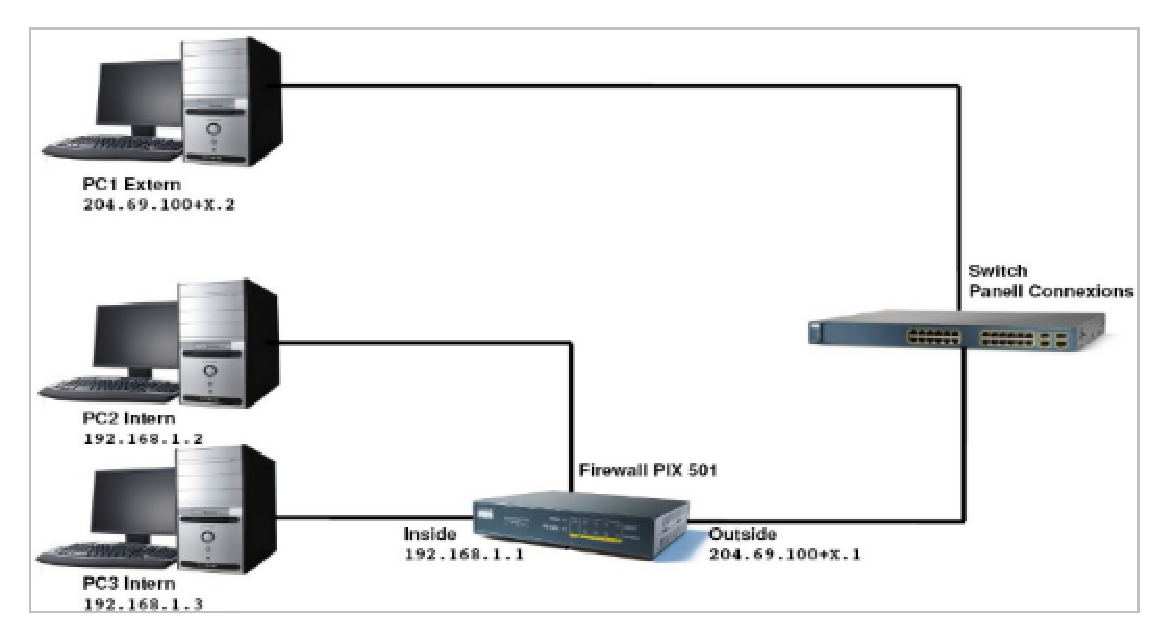
\includegraphics[width=0.9\linewidth]{Figures/firewall_topology.eps}
\fi
\caption{Network topology of the firewalls lab assignment}
\label{fig:firewall_topology}
\end{figure}

We will use FTP to verify that configuration works.
Identify the layer-4 protocol and the port number of FTP.

\section{Adaptive Security Device Manager (ASDM)}

The firewall can be configured using a Java tool which is called Adaptive Security Device Manager (ASDM).
This tool makes it possible to interact with the firewall using a web interface.
Use a windows box to run ASMD.

We will find the ``ASMD launcher'' on the desktop.
The default username and password is blank/blank.
The default IP address is 192.168.1.1 .

The CISCO ASA firewalls assign a ``security level'' to the interfaces.
A security level of 100 means the interface is 100\% trusted.
A security level of 0 means that the interface is not trusted at all.
We will check the interfaces available and their security level.
Discuss the appropriateness of this configuration.

We try to ping between the two PCs connected to the internal interfaces.

\begin{center}
\sffamily\small
\begin{tabular}{>{\columncolor{tablegray}}p{15cm}}

\multicolumn{1}{>{\columncolor{tableorange}}l}{Question}\\
Does it work? Why?\\
\hline
\end{tabular}
\end{center}

\section{Default configuration of the ASA 5505}
The Cisco ASA use the same OS that the other devices used in the previous assignments, the Cisco IOS.
We will click on options$\rightarrow$preferences and activate ``preview commands before sending them to the device''.
This will show us the equivalent commands that would be used on the console to change the configuration.

Explain which is the default configuration of the firewall.
Observe and explain the different aspects that can be configured using the icons on the left hand side of the screen.

\begin{center}
\sffamily\small
\begin{tabular}{>{\columncolor{tablegray}}p{15cm}}

\multicolumn{1}{>{\columncolor{tableorange}}l}{Question}\\
What is the default configuration of Ethernet 0/0 (outside)?\\
\hline
Why do you thing that the router ships with this configuration?\\
\hline
\end{tabular}
\end{center}

We will change the address of the Ethernet 0/0 (outside) interface to 204.69.100+X.1.
Remember that the X is the group number.
We will use a /24 network mask.
Now we connect the outside PC (via switch B) to the outside interface.
We configure the IP of the outside PC to an address of the outside rang and we set the firewall's outside address as the PC's default gateway.

\begin{center}
\sffamily\small
\begin{tabular}{>{\columncolor{tablegray}}p{15cm}}

\multicolumn{1}{>{\columncolor{tableorange}}l}{Question}\\
Can you ping from the outside PC to an inside PC? Why?\\
\hline
Whats the difference compared to the previous case?\\
\hline
\end{tabular}
\end{center}
Look at the syslog (home screen) to answer this questions.

\section{Firewall}
An alternative configuration option is telnet.
We enable the telnet options ASDM configuration$\rightarrow$Properties$\rightarrow$Device Access$\rightarrow$Telnet.
We have to make sure that we have applied the changes (apply and save).
Now we telnet the device and we use \texttt{cisco} (small letters) as a password.

We try the
\begin{lstlisting}
# who
\end{lstlisting}
command to see who is connected to the firewall.
\begin{lstlisting}
# show run
\end{lstlisting}
to see the running configuration.
Find information about telnet and dhcp and explain it.
We also try the commands
\begin{lstlisting}
# show interface
\end{lstlisting}
and
\begin{lstlisting}
# show traffic
\end{lstlisting}
and explain the information that they provide.

Discuss the security implications of connecting using telnet of the console.

\section{The Hosts/Networks table}
In the Network Objects / Groups (Configuration$\rightarrow$Global Objects) we can view, edit, add and delete hosts and networks lists  defined in every interface.
The hosts and networks are organized according to the interface they are connected to (inside/outside).
It is recommended to name all the hosts we are managing.

We add the two internal PCs by clicking on ``add network object''.
The mask is 255.255.255.255, as it is a single host.
Add also the external PC.
We apply and save.

\section{Access Rules}
The access rules make it possible to establish security policies as a list of rules.
The tables to specify how a computer interacts with another by allowing and denying specific services and protocols.

We try to connect from the inside PC to the outside PC and explain the behaviour and the default ``Access Rules'' table for the inside interface.

The rules are examined sequentially until one of the applies.
If the first rule applies, the second is not checked.
If the first rule does not apply, then the second is checked.
The process is repeated until one of the rules applies.
\begin{center}
\sffamily\small
\begin{tabular}{>{\columncolor{tablegray}}p{15cm}}

\multicolumn{1}{>{\columncolor{tableorange}}l}{Question}\\
The last rule is ``any to any deny''. Why?\\
\hline
\end{tabular}
\end{center}

The first rule allows traffic from any IP source to any IP destination if the destination interface has a lower security level.
If this rule does not apply, the second rule is examined.
The second rule always applies and discards the packet.

We will observe and explain the rules for the traffic arriving to the external interfaces.
To understand the rules, we will pay attention to the graphical diagrams offered by the software.`

We will install and configure the FTP server to the external computer.
Remember that it is needed to add a folder.
\begin{center}
\sffamily\small
\begin{tabular}{>{\columncolor{tablegray}}p{15cm}}

\multicolumn{1}{>{\columncolor{tableorange}}l}{Question}\\
Is it possible to access the FTP server from the internal computers?\\
\hline
\end{tabular}
\end{center}

Use the rules to deny the access to the FTP server to one of the internal computers and allow access to the other.
Observe the log messages to verify that access is being denied.
Each time that you change the configuration and try to access to the ftp server, clean the browser cache.

\section{Translation Rules}

The ASA 5505 supports both network address translation (NAT) which is a one-to-one address translation (one inside to one outside) and port address translation (PAT) which is a many-to-one address translation.

Look at the default configuration for the translation rules.
\begin{center}
\sffamily\small
\begin{tabular}{>{\columncolor{tablegray}}p{15cm}}

\multicolumn{1}{>{\columncolor{tableorange}}l}{Question}\\
How does this configuration affect outgoing traffic?\\
\hline
What is the IP address used after the packets traverse the firewall?\\
\hline
\end{tabular}
\end{center}

\section{Monitoring}
The ASDM can be used for network monitoring.
It allows to select the message supervising level.
Check the telnet connections and connected users using the options of the menu on the left.

There is also a tool to generate graphs such as traffic, memory and CPU.
Look at some of the graphs and explain them.

\section{Case Study}

An enterprise has C class network 204.69.100+X.0 and wants securely connect their internal network to an external network.
The address of the outside firewall interface is 204.69.100+X.1.

In the internal network there is an FTP server with address 192.168.1.4 that needs to be accessed from the outside network using the address 204.69.100+X.4.

The other requirements are that internal users must be able to ping external devices, but not the other way around.

We will configure the firewall to satisfy the above requirements using the command line interface (CLI).
Explain the commands that have been used as well as the tests performed to verify the correctness of the configuration.
